\section{Arquitectura de Software}

El desarrollo de Navindoor se ha dividido en módulos claramente diferenciados, que siguen los pasos para el posicionamiento mencionado en la introducción. A continuación describiremos cada una de ellas.
% ----------------------------------------------------------------------
\subsection{Planimetría}
\begin{figure}
    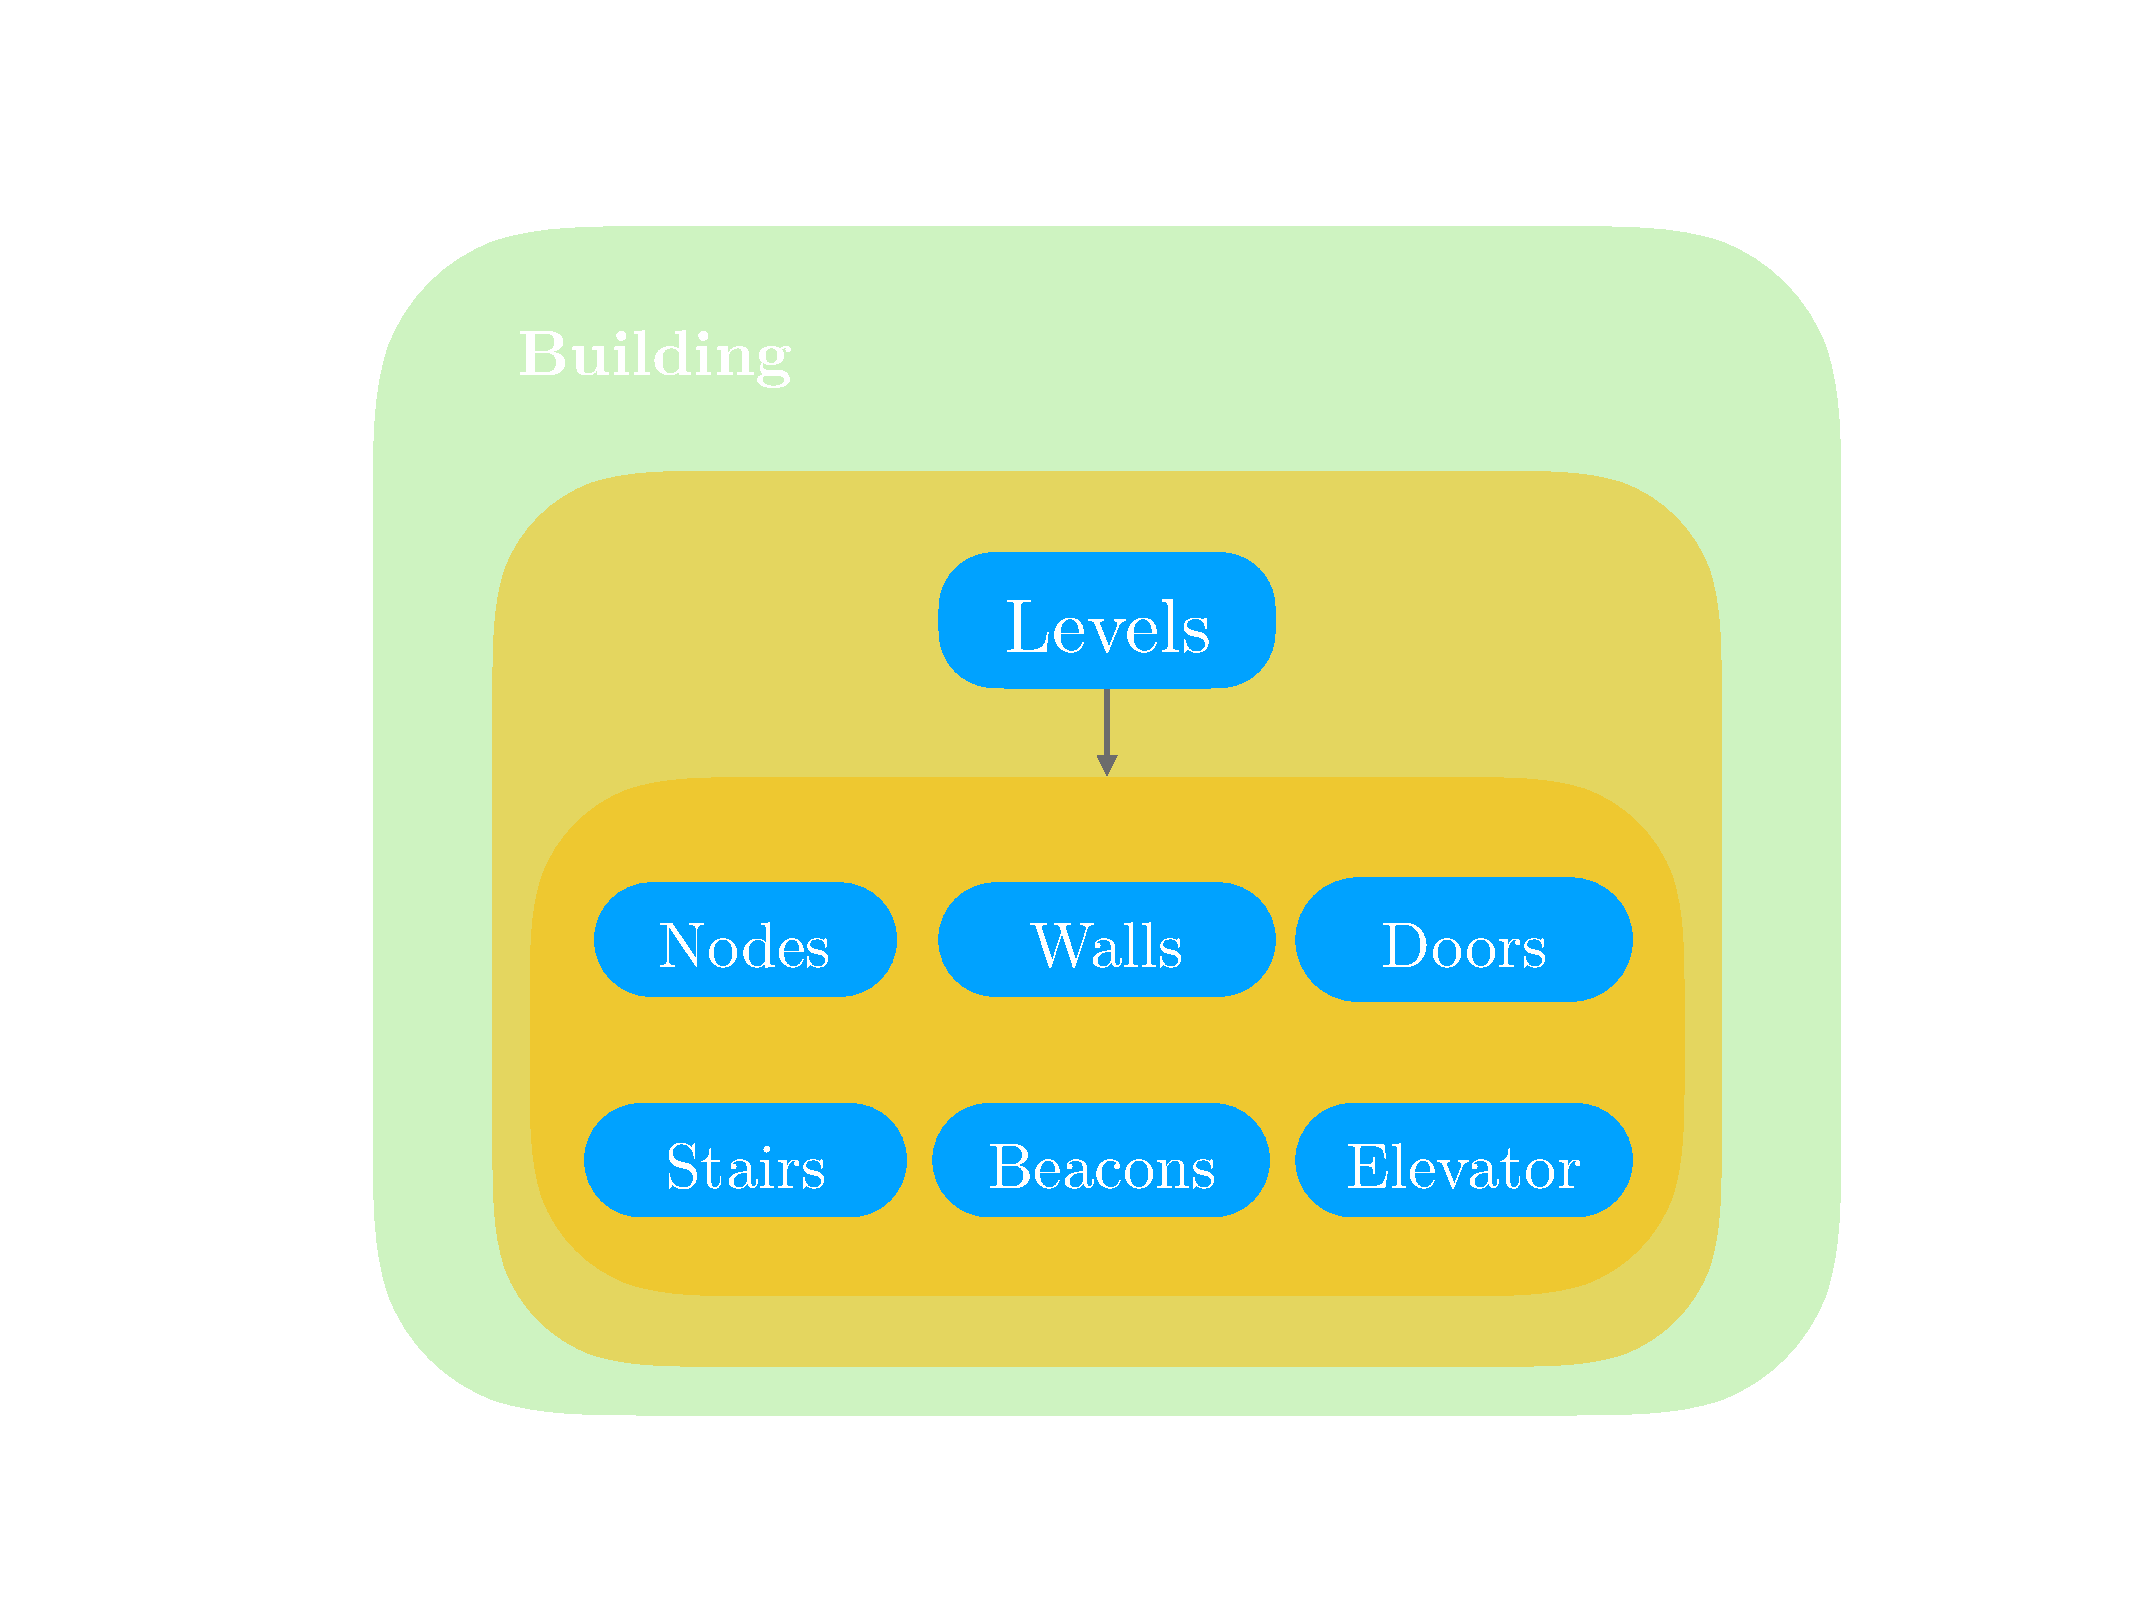
\includegraphics[width=1.0\columnwidth]{img/Design/1.pdf}
    \caption[]{Visualización de la Facultad de ingeniería}
\end{figure}
% ----------------------------------------------------------------------
\subsection{Trayectorias}
\begin{figure}
    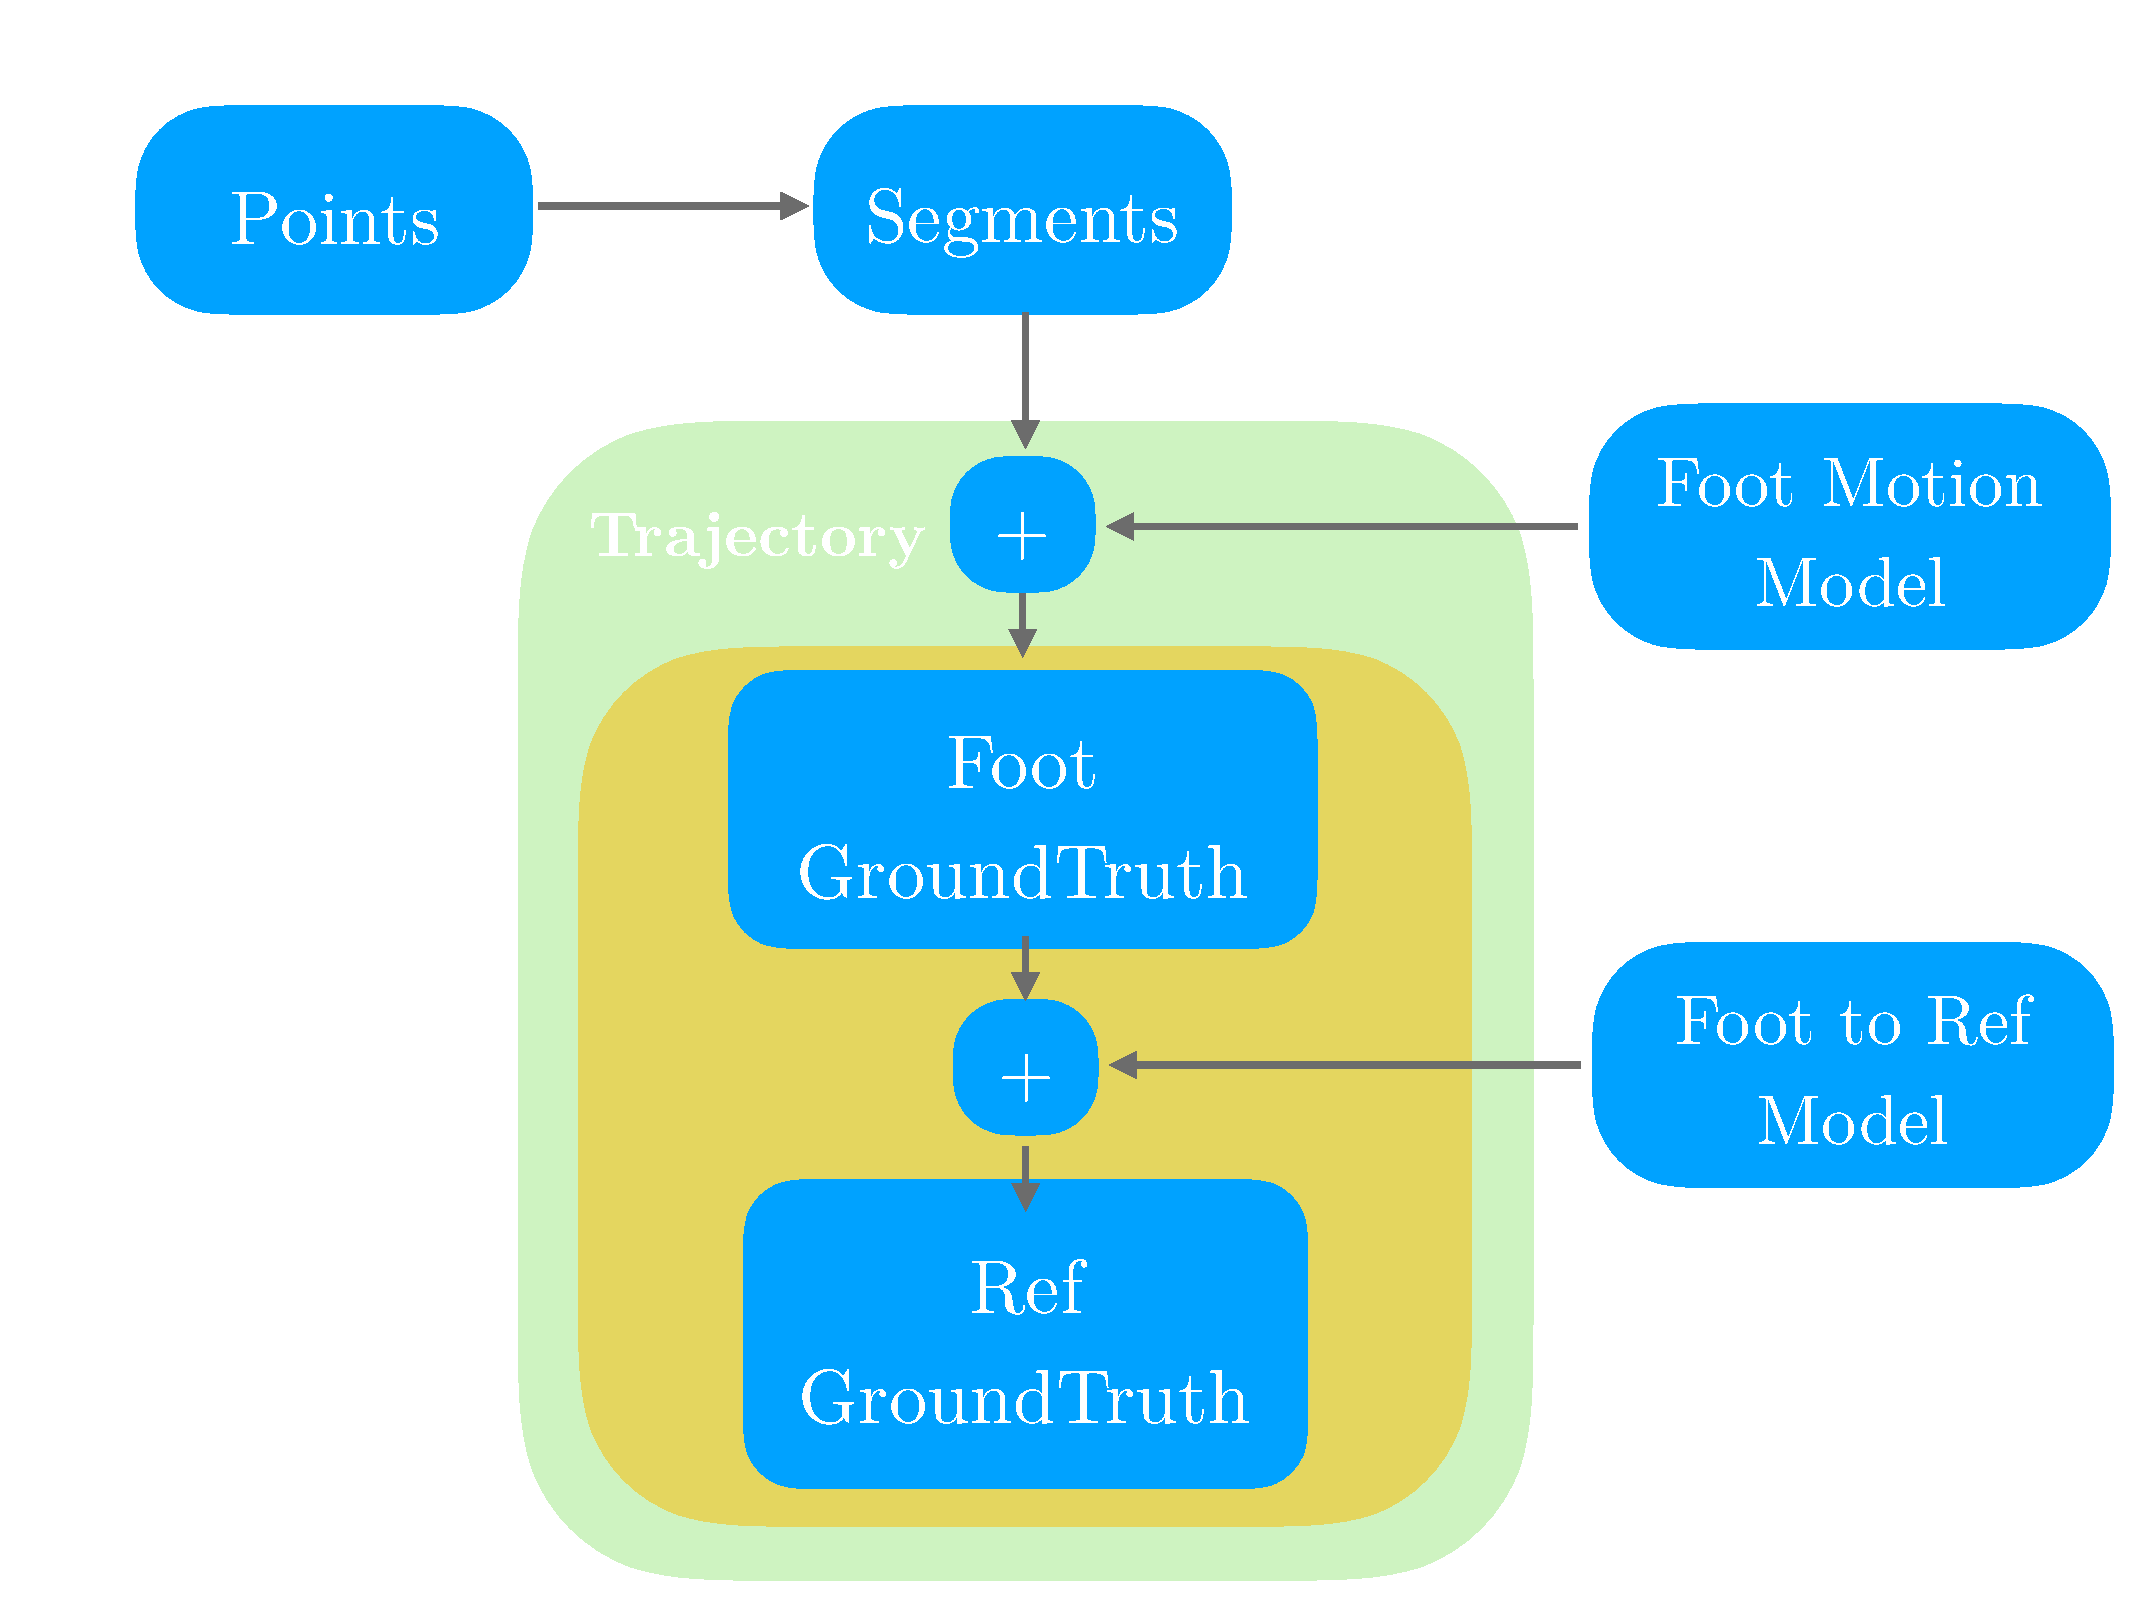
\includegraphics[width=1.0\columnwidth]{img/Design/2.pdf}
    \caption[]{Visualización de la Facultad de ingeniería}
\end{figure}
% ----------------------------------------------------------------------
\subsection{Señales}
Para la representación de las  señales se ha creado un objeto MATLAB ...
\begin{figure}
    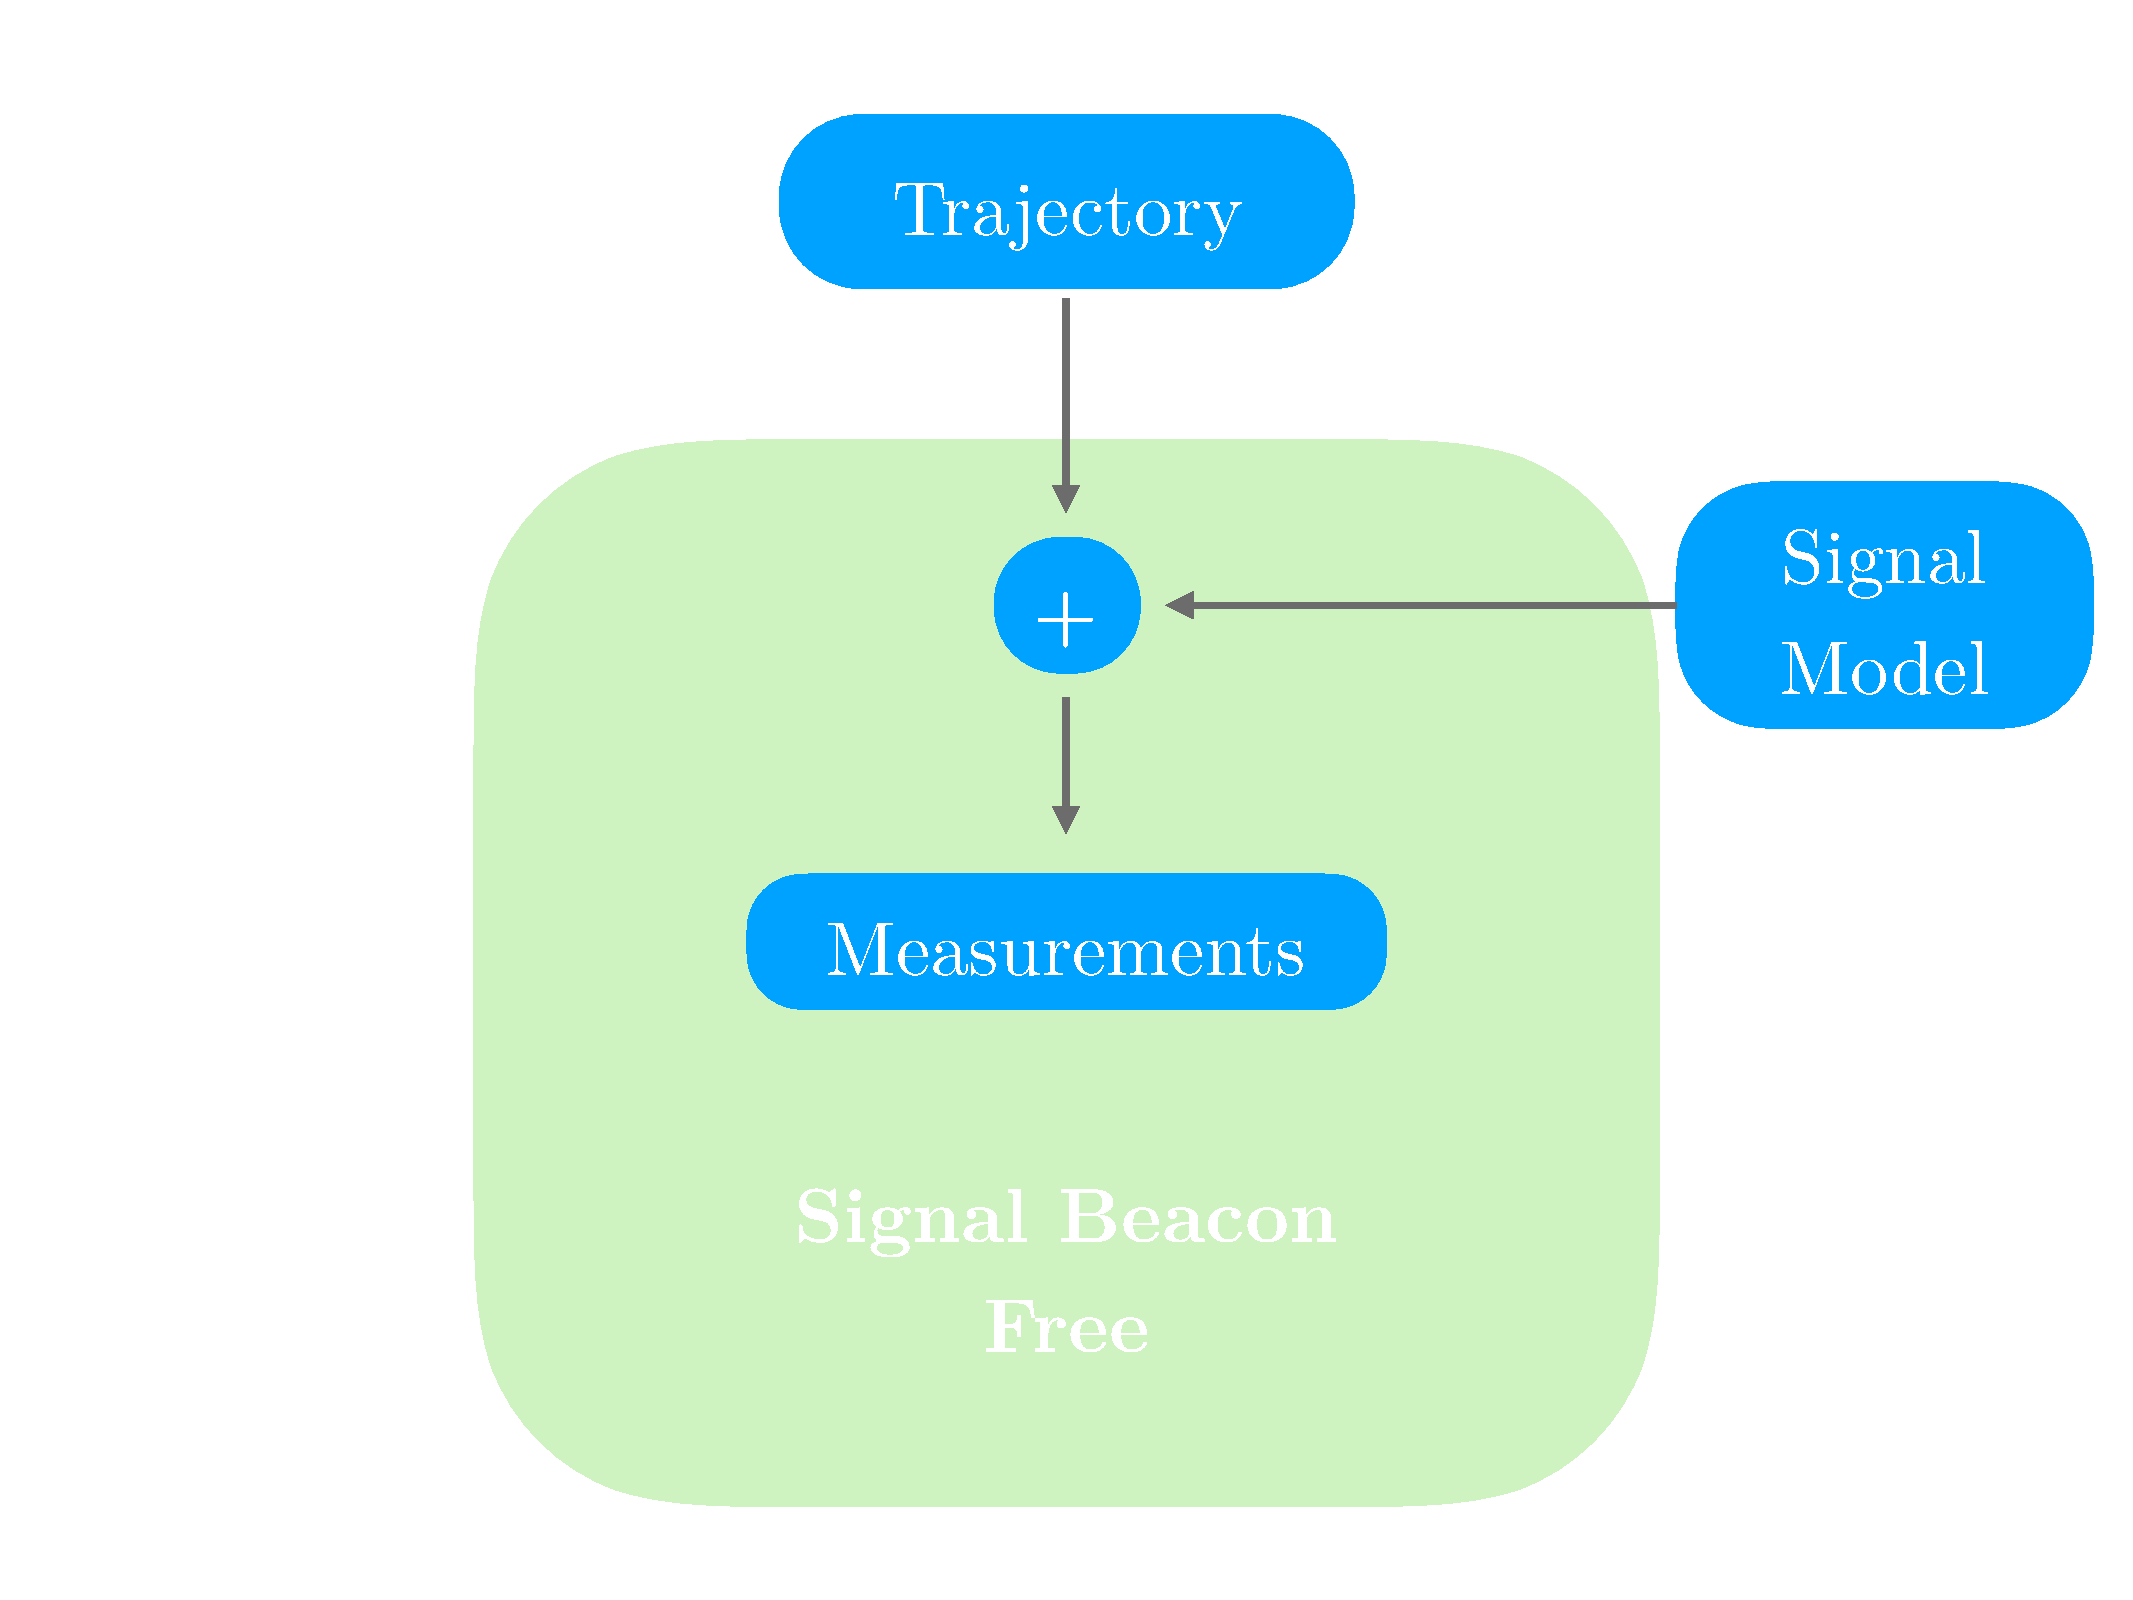
\includegraphics[width=1.0\columnwidth]{img/Design/3.pdf}
    \caption[]{Visualización de la Facultad de ingeniería}
\end{figure}
\begin{figure}
    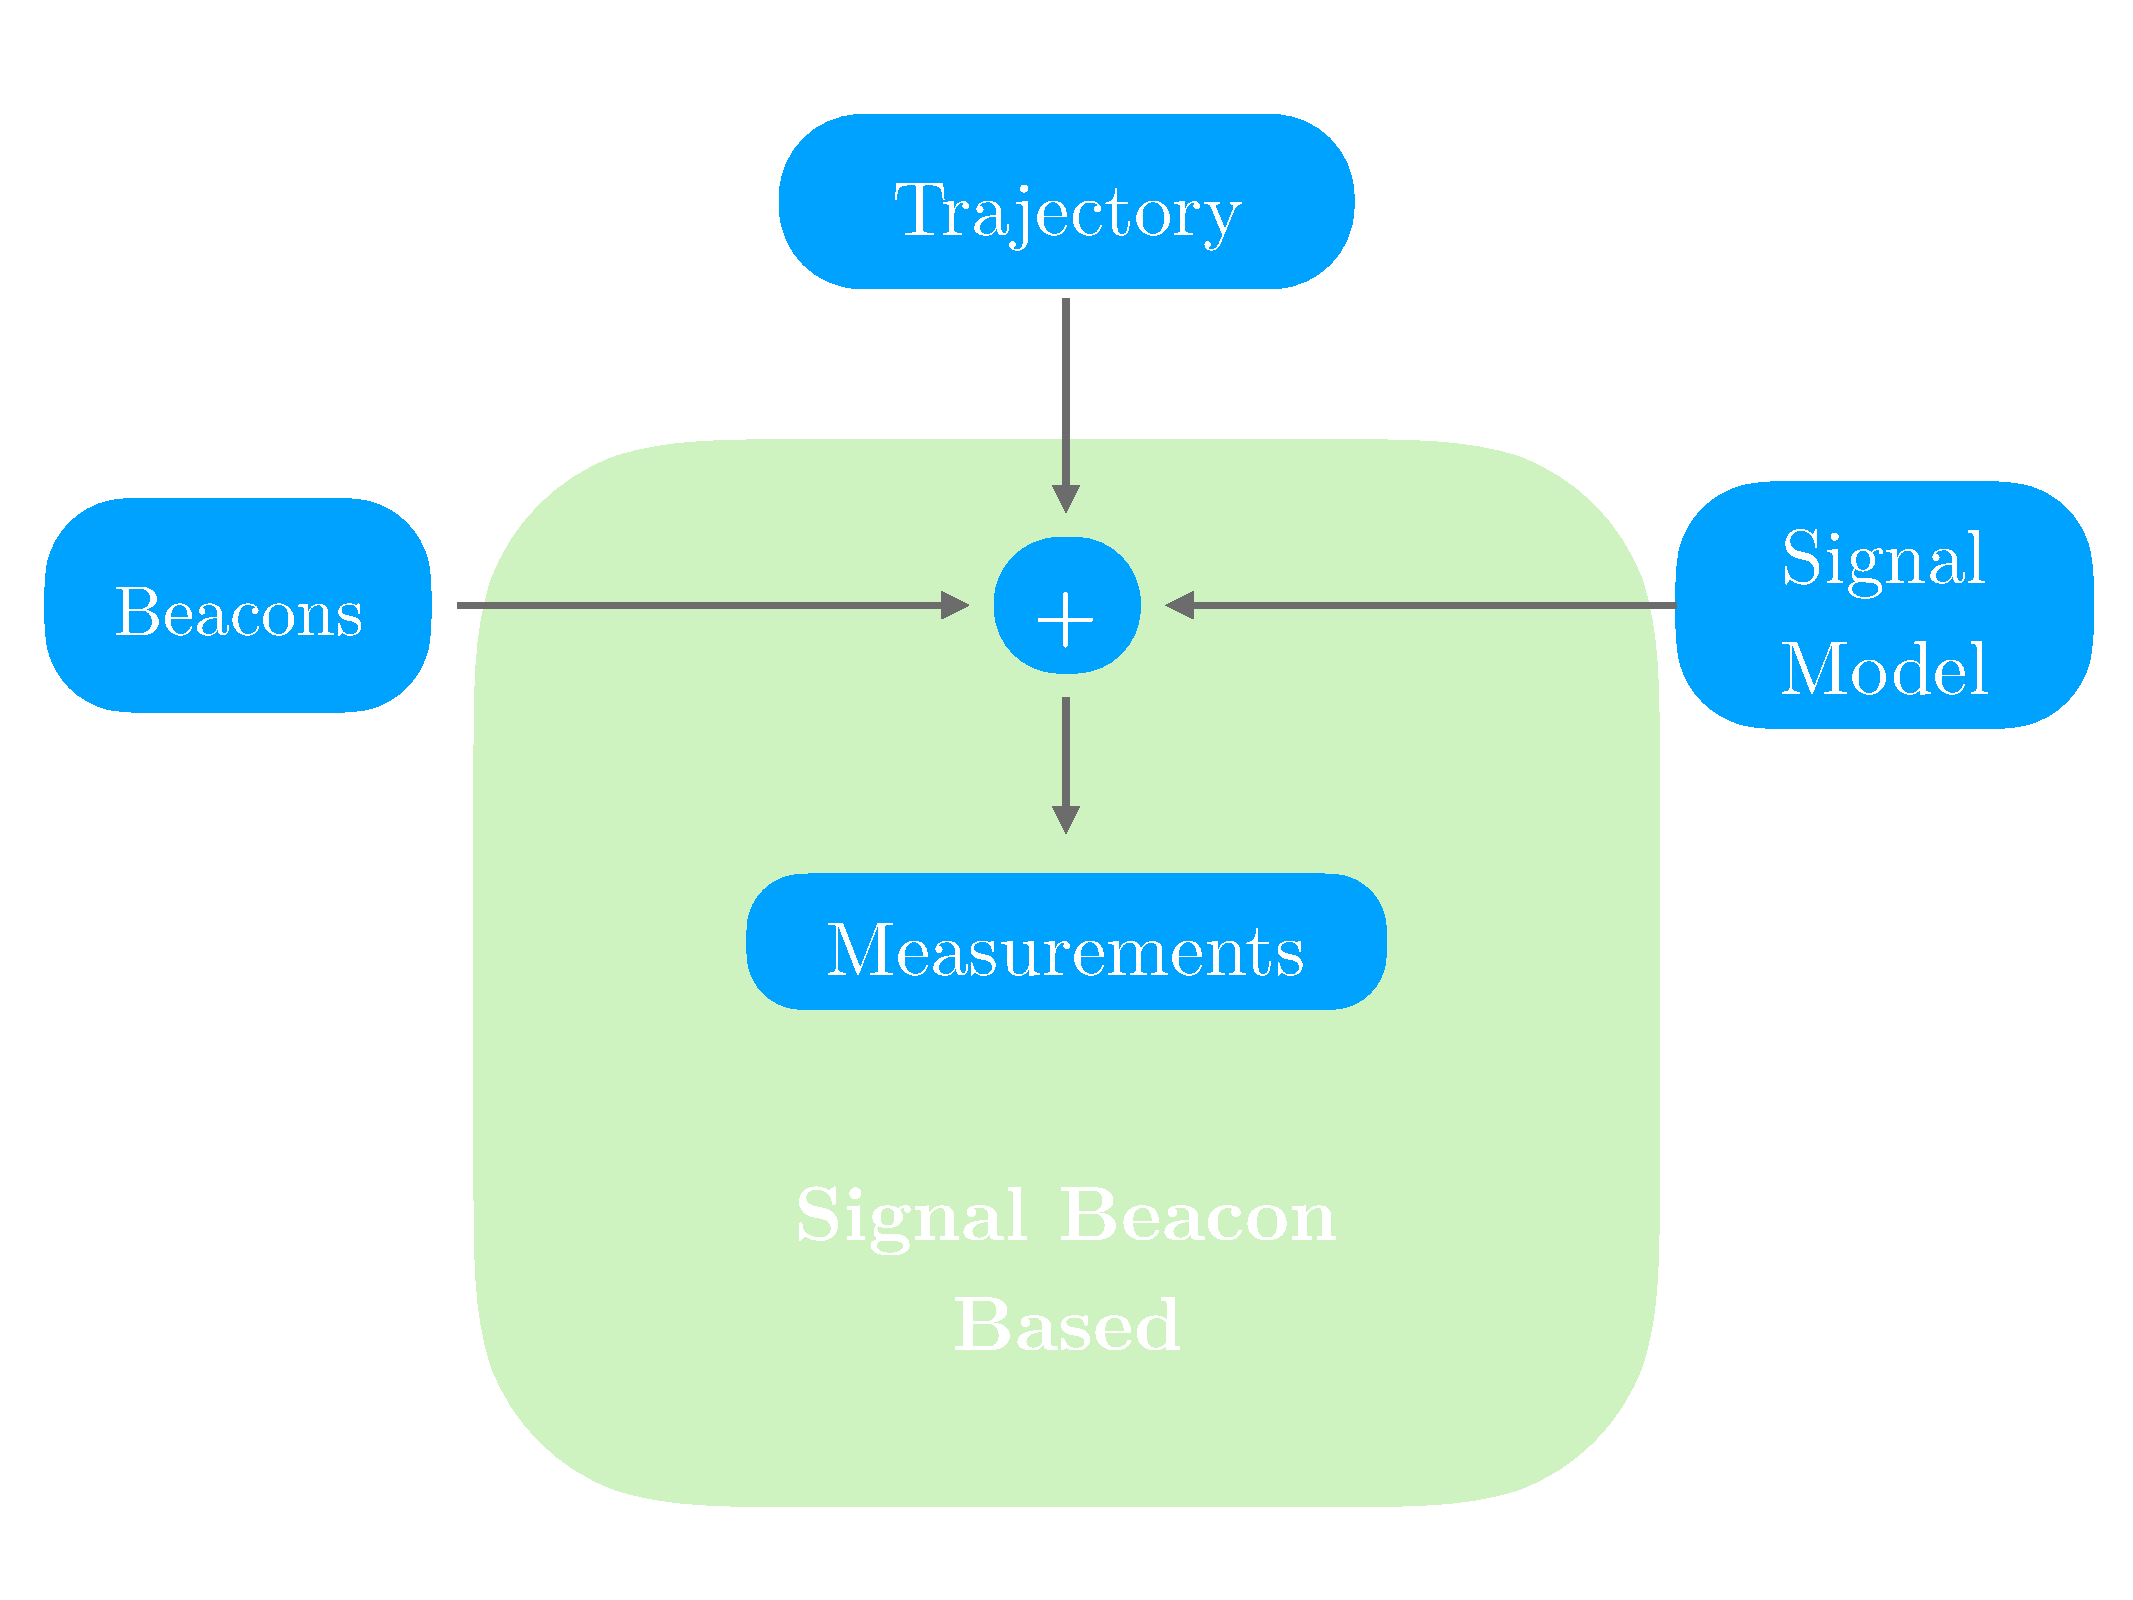
\includegraphics[width=1.0\columnwidth]{img/Design/4.pdf}
    \caption[]{Visualización de la Facultad de ingeniería}
\end{figure}
% ----------------------------------------------------------------------
\subsection{Procesamiento}
\begin{figure}
    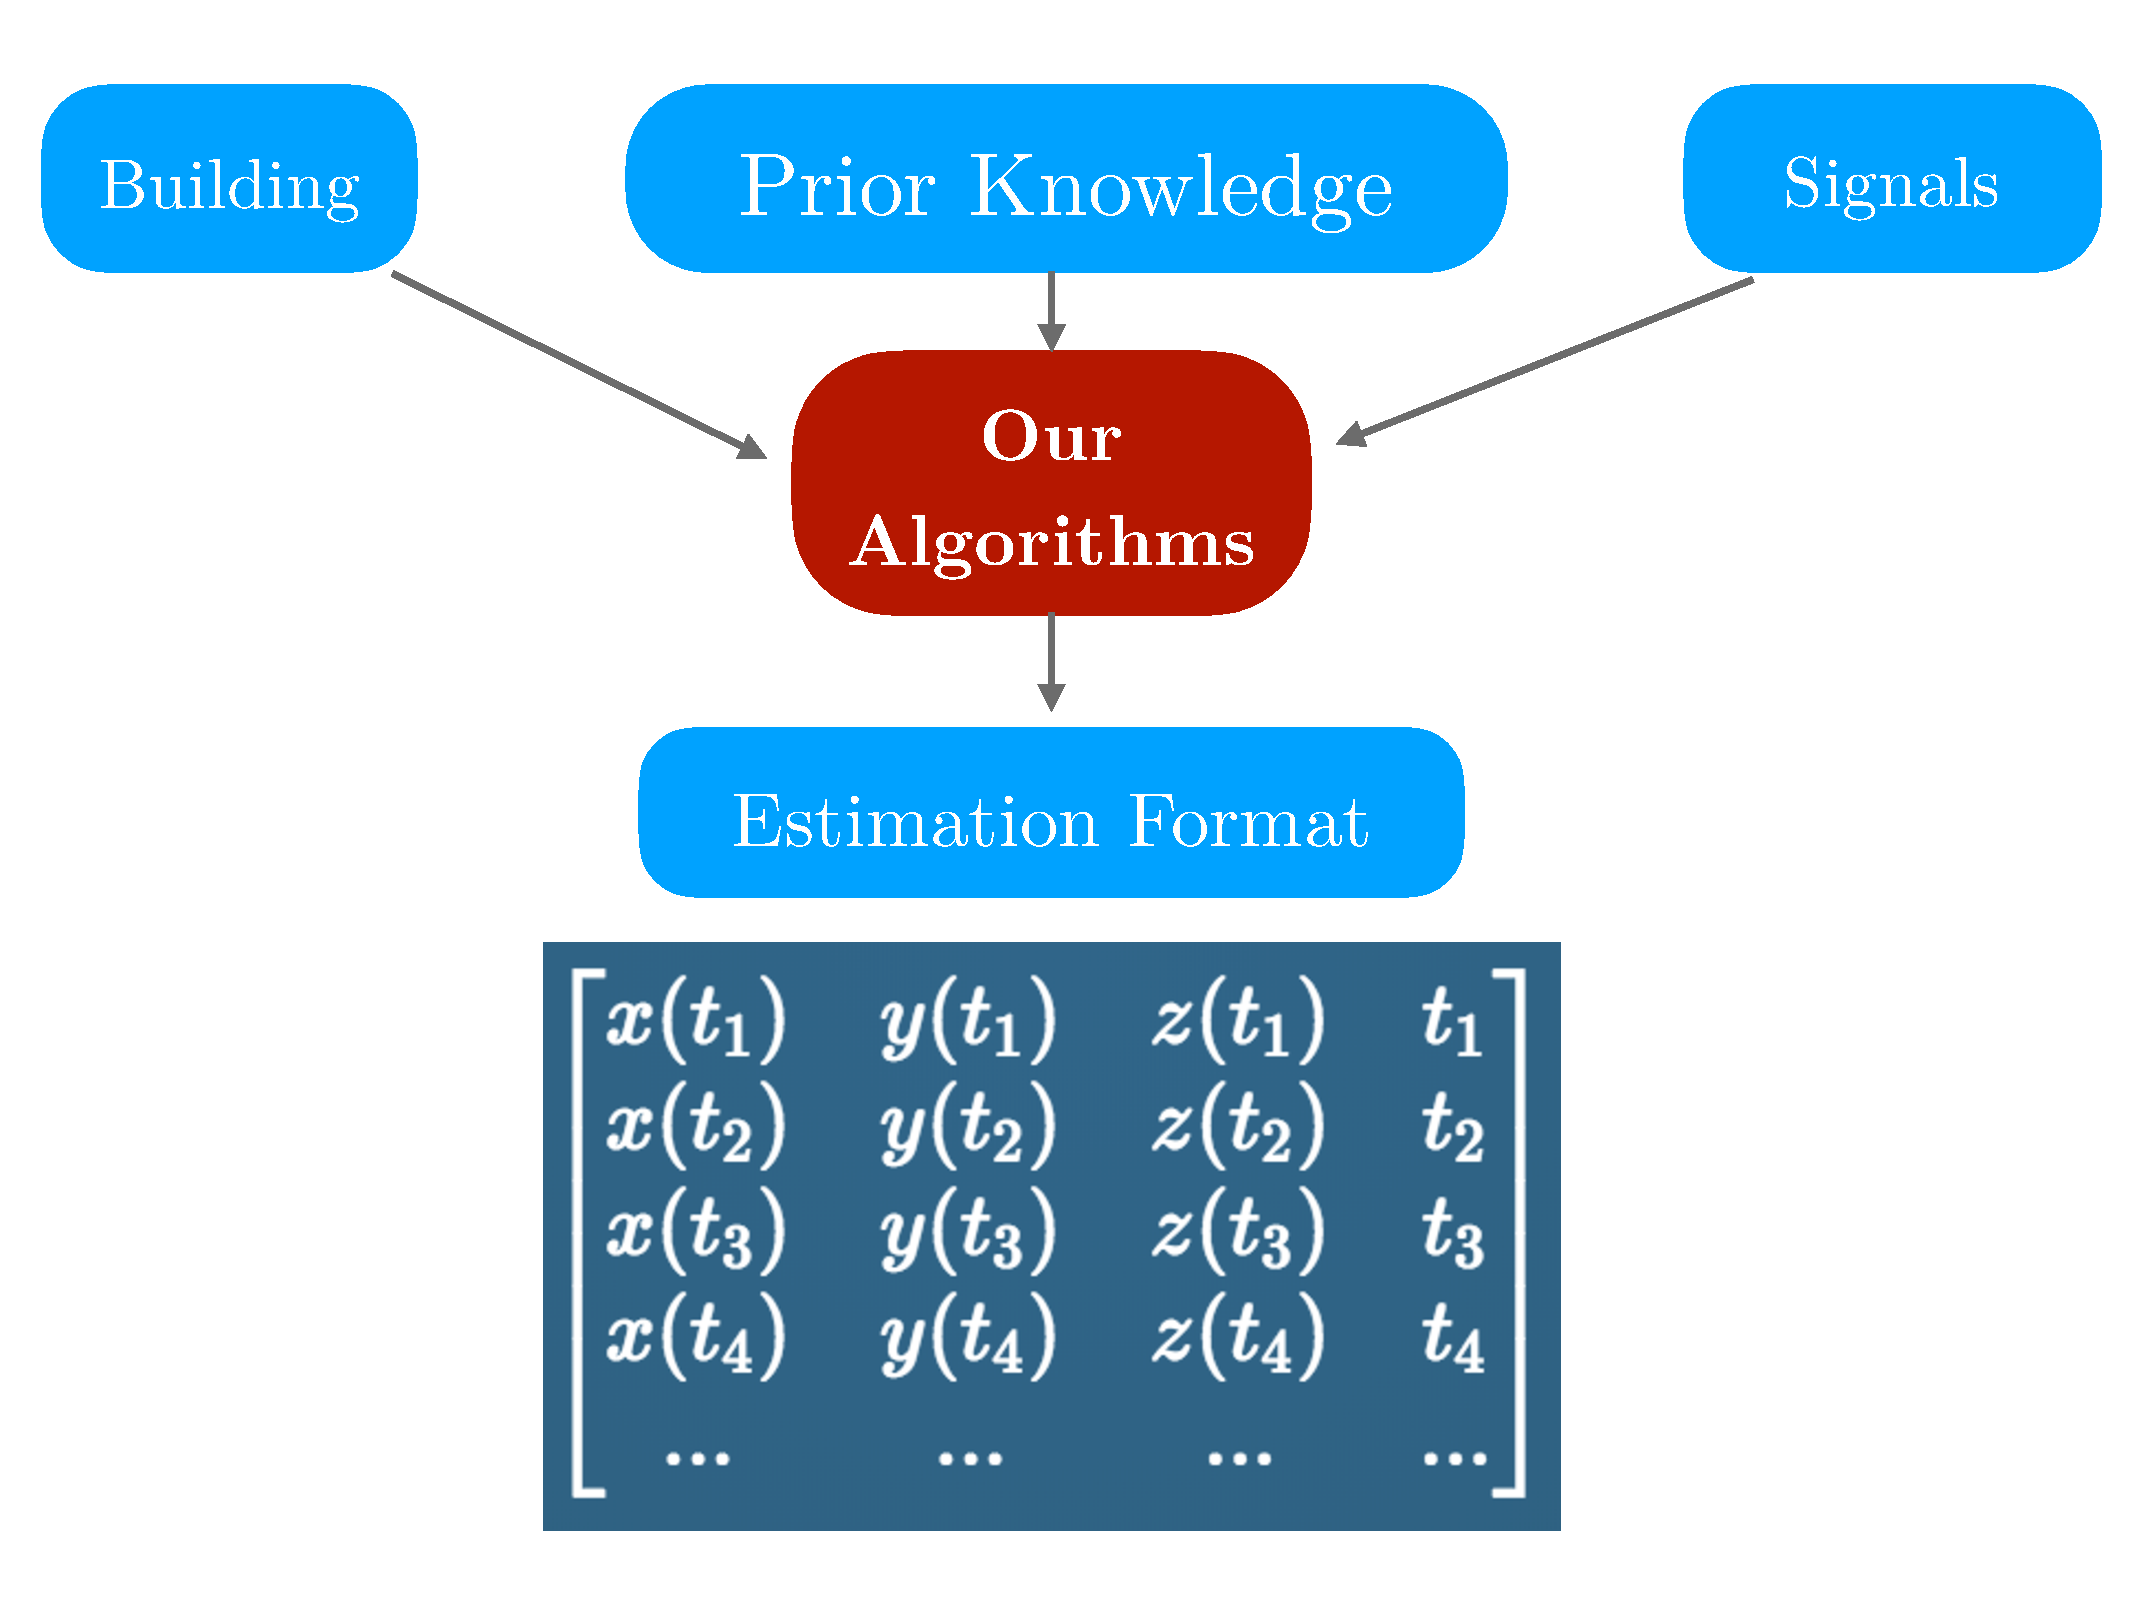
\includegraphics[width=1.0\columnwidth]{img/Design/5.pdf}
    \caption[]{Visualización de la Facultad de ingeniería}
\end{figure}
% ----------------------------------------------------------------------
\subsection{Comparación}